%----------------------------------------------------------------------------------------
%	PACKAGES AND THEMES
%----------------------------------------------------------------------------------------
\documentclass[aspectratio=169,xcolor=dvipsnames]{beamer}
\usetheme{Simple}

\usepackage{bm}
\usepackage{amsmath}
\usepackage{mathabx}
\usepackage{hyperref}
\usepackage{graphicx} % Allows including images
\usepackage{booktabs} % Allows the use of \toprule, \midrule and \bottomrule in tables
\usepackage{listings} % Inline code and codeblocks
\usepackage{xparse}   % For verbatim writing
\usepackage{caption}
\usepackage{tikz}
\usetikzlibrary{bayesnet}
\usetikzlibrary{arrows}

\lstset{language=C,keywordstyle={\bfseries \color{blue}}}

%----------------------------------------------------------------------------------------
%	TITLE PAGE
%----------------------------------------------------------------------------------------

% The title
\title[short title]{Multivariate Analysis}
\subtitle{Estimation with Missing Not at Random Data}

\author[GB] {Guillaume Blanc, Phd. Candidate, \\ University of Geneva}

\date{{\large February 2022}} % Date, can be changed to a custom date


%----------------------------------------------------------------------------------------
%	PRESENTATION SLIDES
%----------------------------------------------------------------------------------------

\begin{document}




\begin{frame}
    % Print the title page as the first slide
    \titlepage
\end{frame}

%------------------------------------------------

\begin{frame}{Multivariate Data with Missing Values}
    \noindent\begin{minipage}[t]{0.65\linewidth}
    \begin{figure}
        \centering
        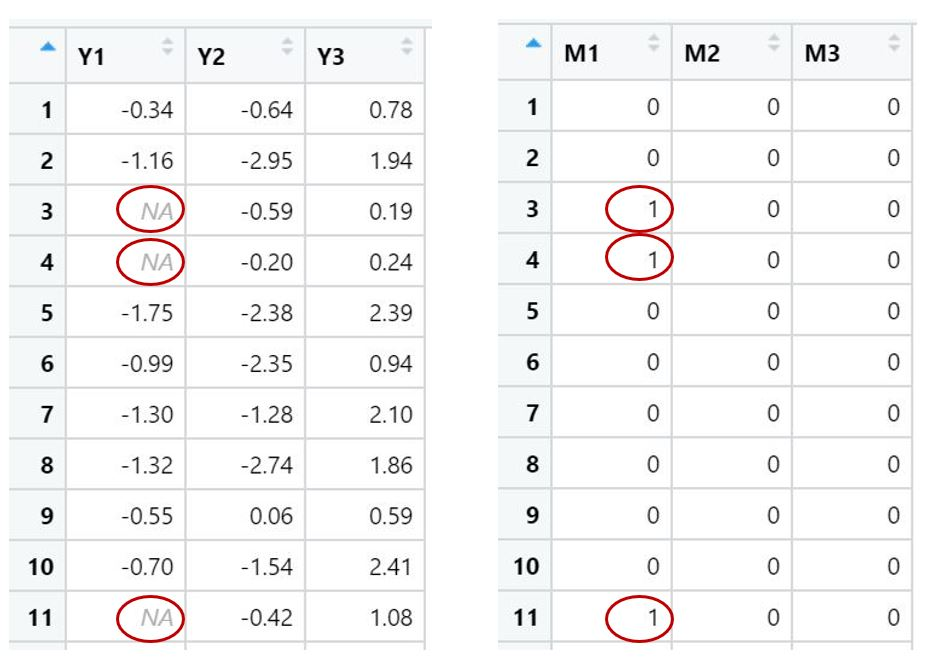
\includegraphics[width=.85\textwidth]{images/missin_ex.JPG}
        \caption{Data with missing values and the mask.}
    \end{figure}
    \end{minipage}
    \noindent\begin{minipage}[t]{0.33\linewidth}
        \fontsize{11pt}{15}\selectfont
        \vspace{.3cm}
        \noindent
        \textbf{Goal}: estimate $\bm\mu$

        \noindent
        \textbf{Problem}: missing values

        \vspace{1cm}
        \noindent
        \textbf{Solution}: 
        \begin{enumerate}
            \item Impute by the mean (?!)
            \item Correct the bias.
        \end{enumerate}

        \noindent
        \textbf{Requires}:
        \begin{itemize}%[label={--}]
            \item Generative model for $\bm Y$
            \item Missingness mechanism
        \end{itemize}
    \end{minipage}
\end{frame}

\begin{frame}{Experiment: Imputation by the Mean}
\noindent\begin{minipage}[t]{0.35\linewidth}
    \vspace{1cm}
    \textbf{Experiment}: Simulate 1000 datasets with missing data. For each, get estimates of $\mu_1$.

    \noindent \textbf{Two settings}:
    \begin{itemize}
        \item {MCAR} : Missing Completely at Random.
        \item {Truncated} : Only smallest 50\% of the data are observed.
    \end{itemize}
\end{minipage}
\noindent\begin{minipage}[t]{0.63\linewidth}
    \begin{figure}
        \centering
        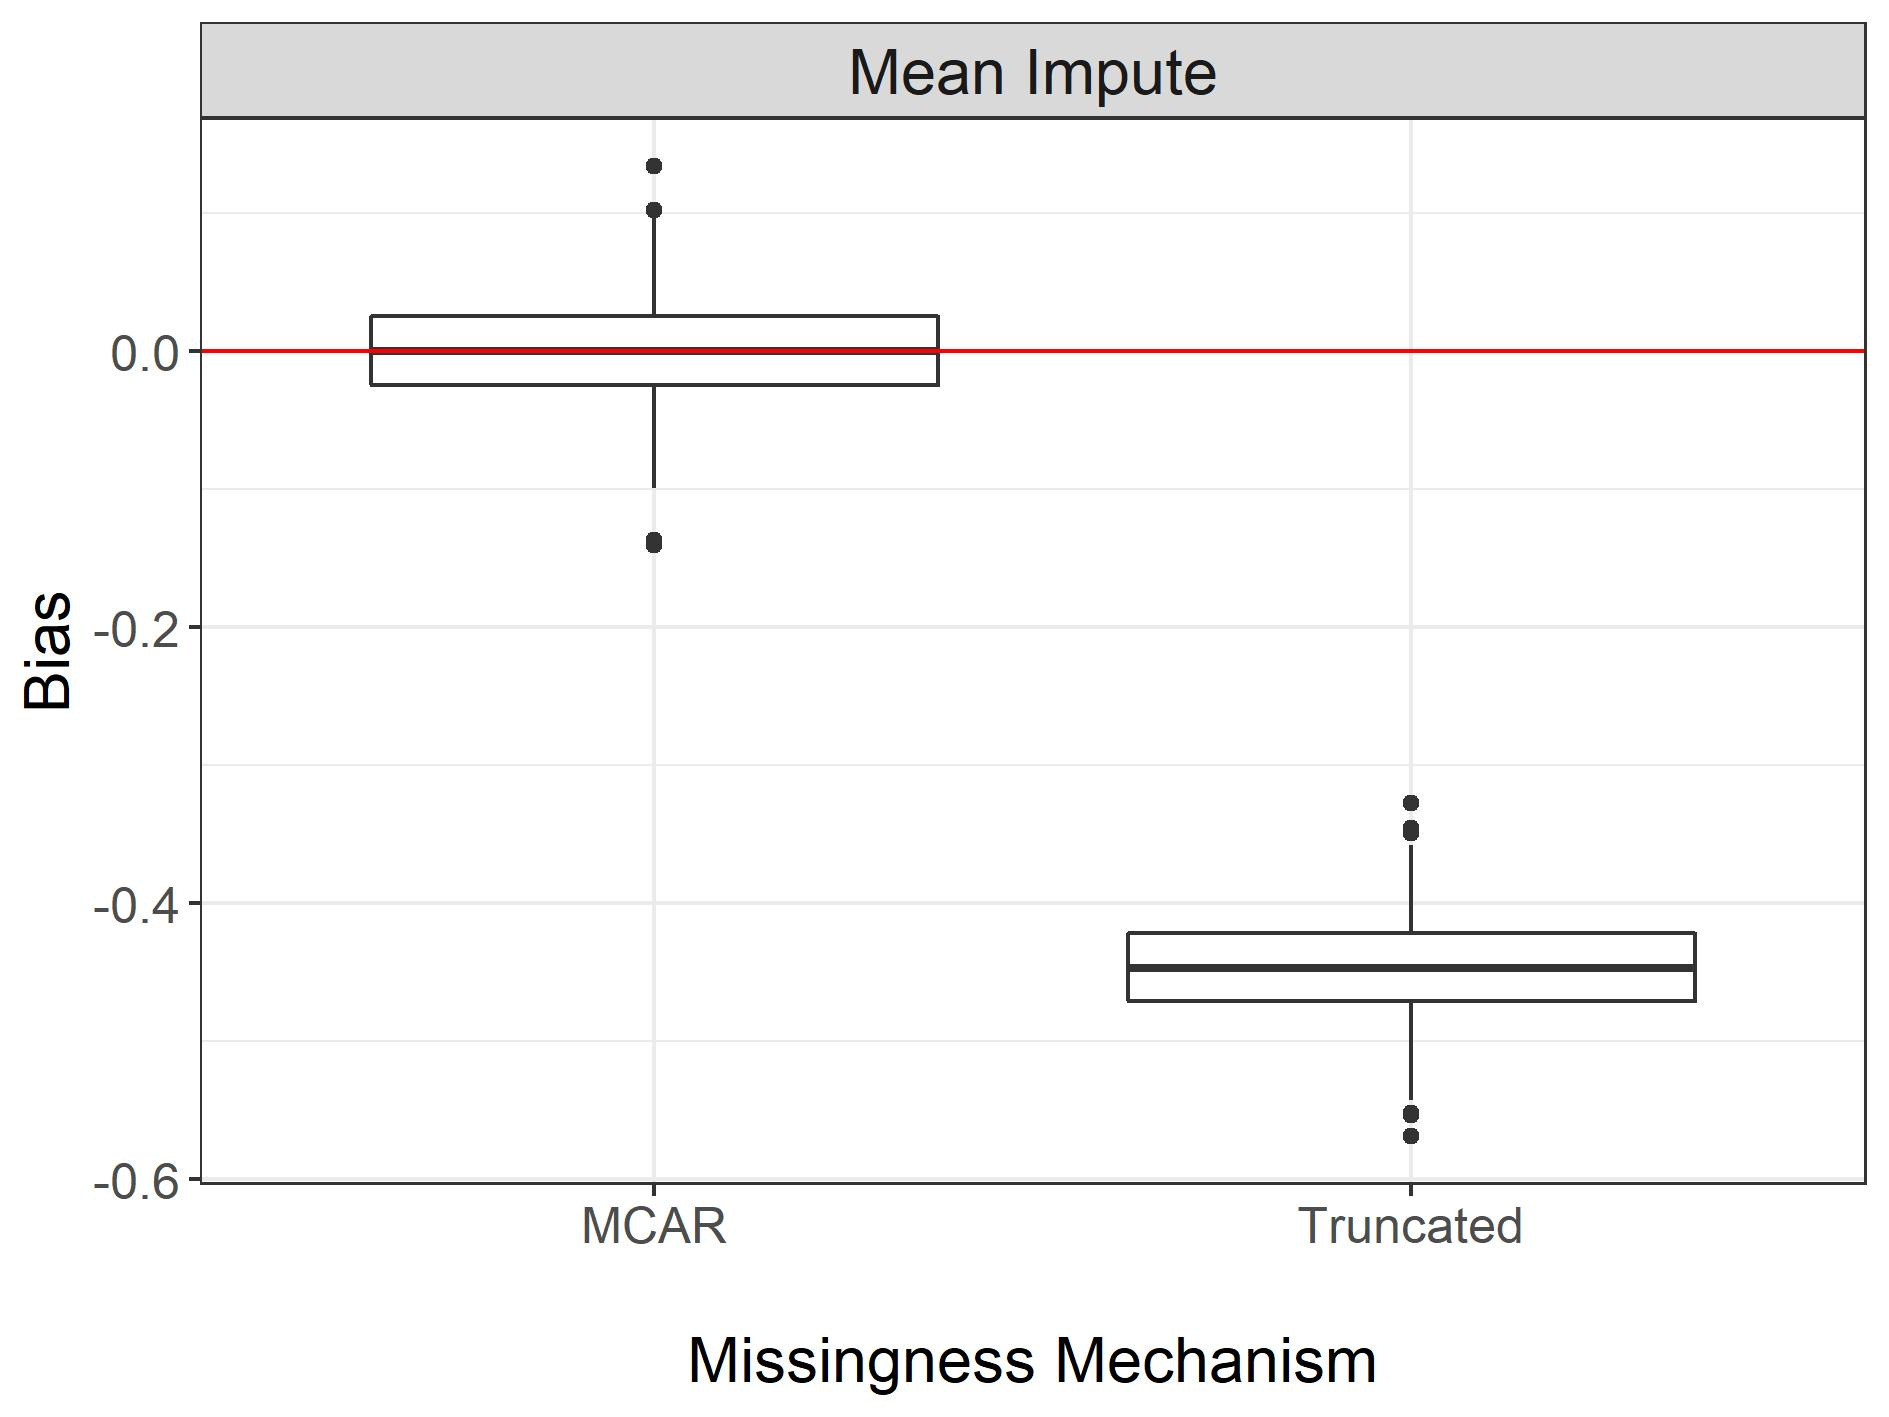
\includegraphics[width=.95\textwidth]{images/plot_bias_1.jpg}
    \end{figure}
\end{minipage}
\end{frame}

\begin{frame}{Generative Model for $\bm Y$: Factor Analysis / PPCA}
\noindent\begin{minipage}[t]{0.48\linewidth}
    \begin{figure}
        \tikz{
        % nodes
        \node[obs] (Yobs) {$\underset{[p]}{\boldsymbol Y}$};%
        \node[latent,above=of Yobs] (Z) {$\underset{[q]}{\boldsymbol Z}$}; %
        \node[const,left = of Z] (parY) {$\boldsymbol \Lambda, \boldsymbol\mu, \boldsymbol \psi$}; %
        % plate
        \plate [inner sep=.3cm,xshift=.02cm,yshift=.2cm] {plate1} {(Z)(Yobs)} {$n$}; %
        % edges
        \edge{Z,parY}{Yobs};
        }
    \caption{Generative model of the data.}
    \end{figure}
\end{minipage}
\fontsize{10pt}{10}\selectfont
\noindent\begin{minipage}[t]{0.48\linewidth}
\vspace{1cm}
\noindent \textbf{Assumptions}: for $j, j' =1, \dots, p$:
\vspace{.5cm}
\begin{itemize}
    \item $Y_j^{obs} \perp Y_{j'}^{obs}|\boldsymbol Z$ whenever $j\neq j'$,
    \item $Y_j^{obs}|\boldsymbol Z = \boldsymbol z \sim N(\boldsymbol z^\top \boldsymbol \Lambda_{j\cdot} + \mu_j,\, \psi_j)$.
\end{itemize}
\vspace{1cm}
\textbf{Consequence}: the marginal distribution is
    $$\boldsymbol Y^{obs} \sim MN(\boldsymbol \mu,\, \boldsymbol \Lambda \boldsymbol \Lambda^\top  + \boldsymbol \psi).$$
\end{minipage}
\end{frame}

\begin{frame}{Bias Correction with Known Missingness Mechanism}
    \begin{figure}
        \centering
        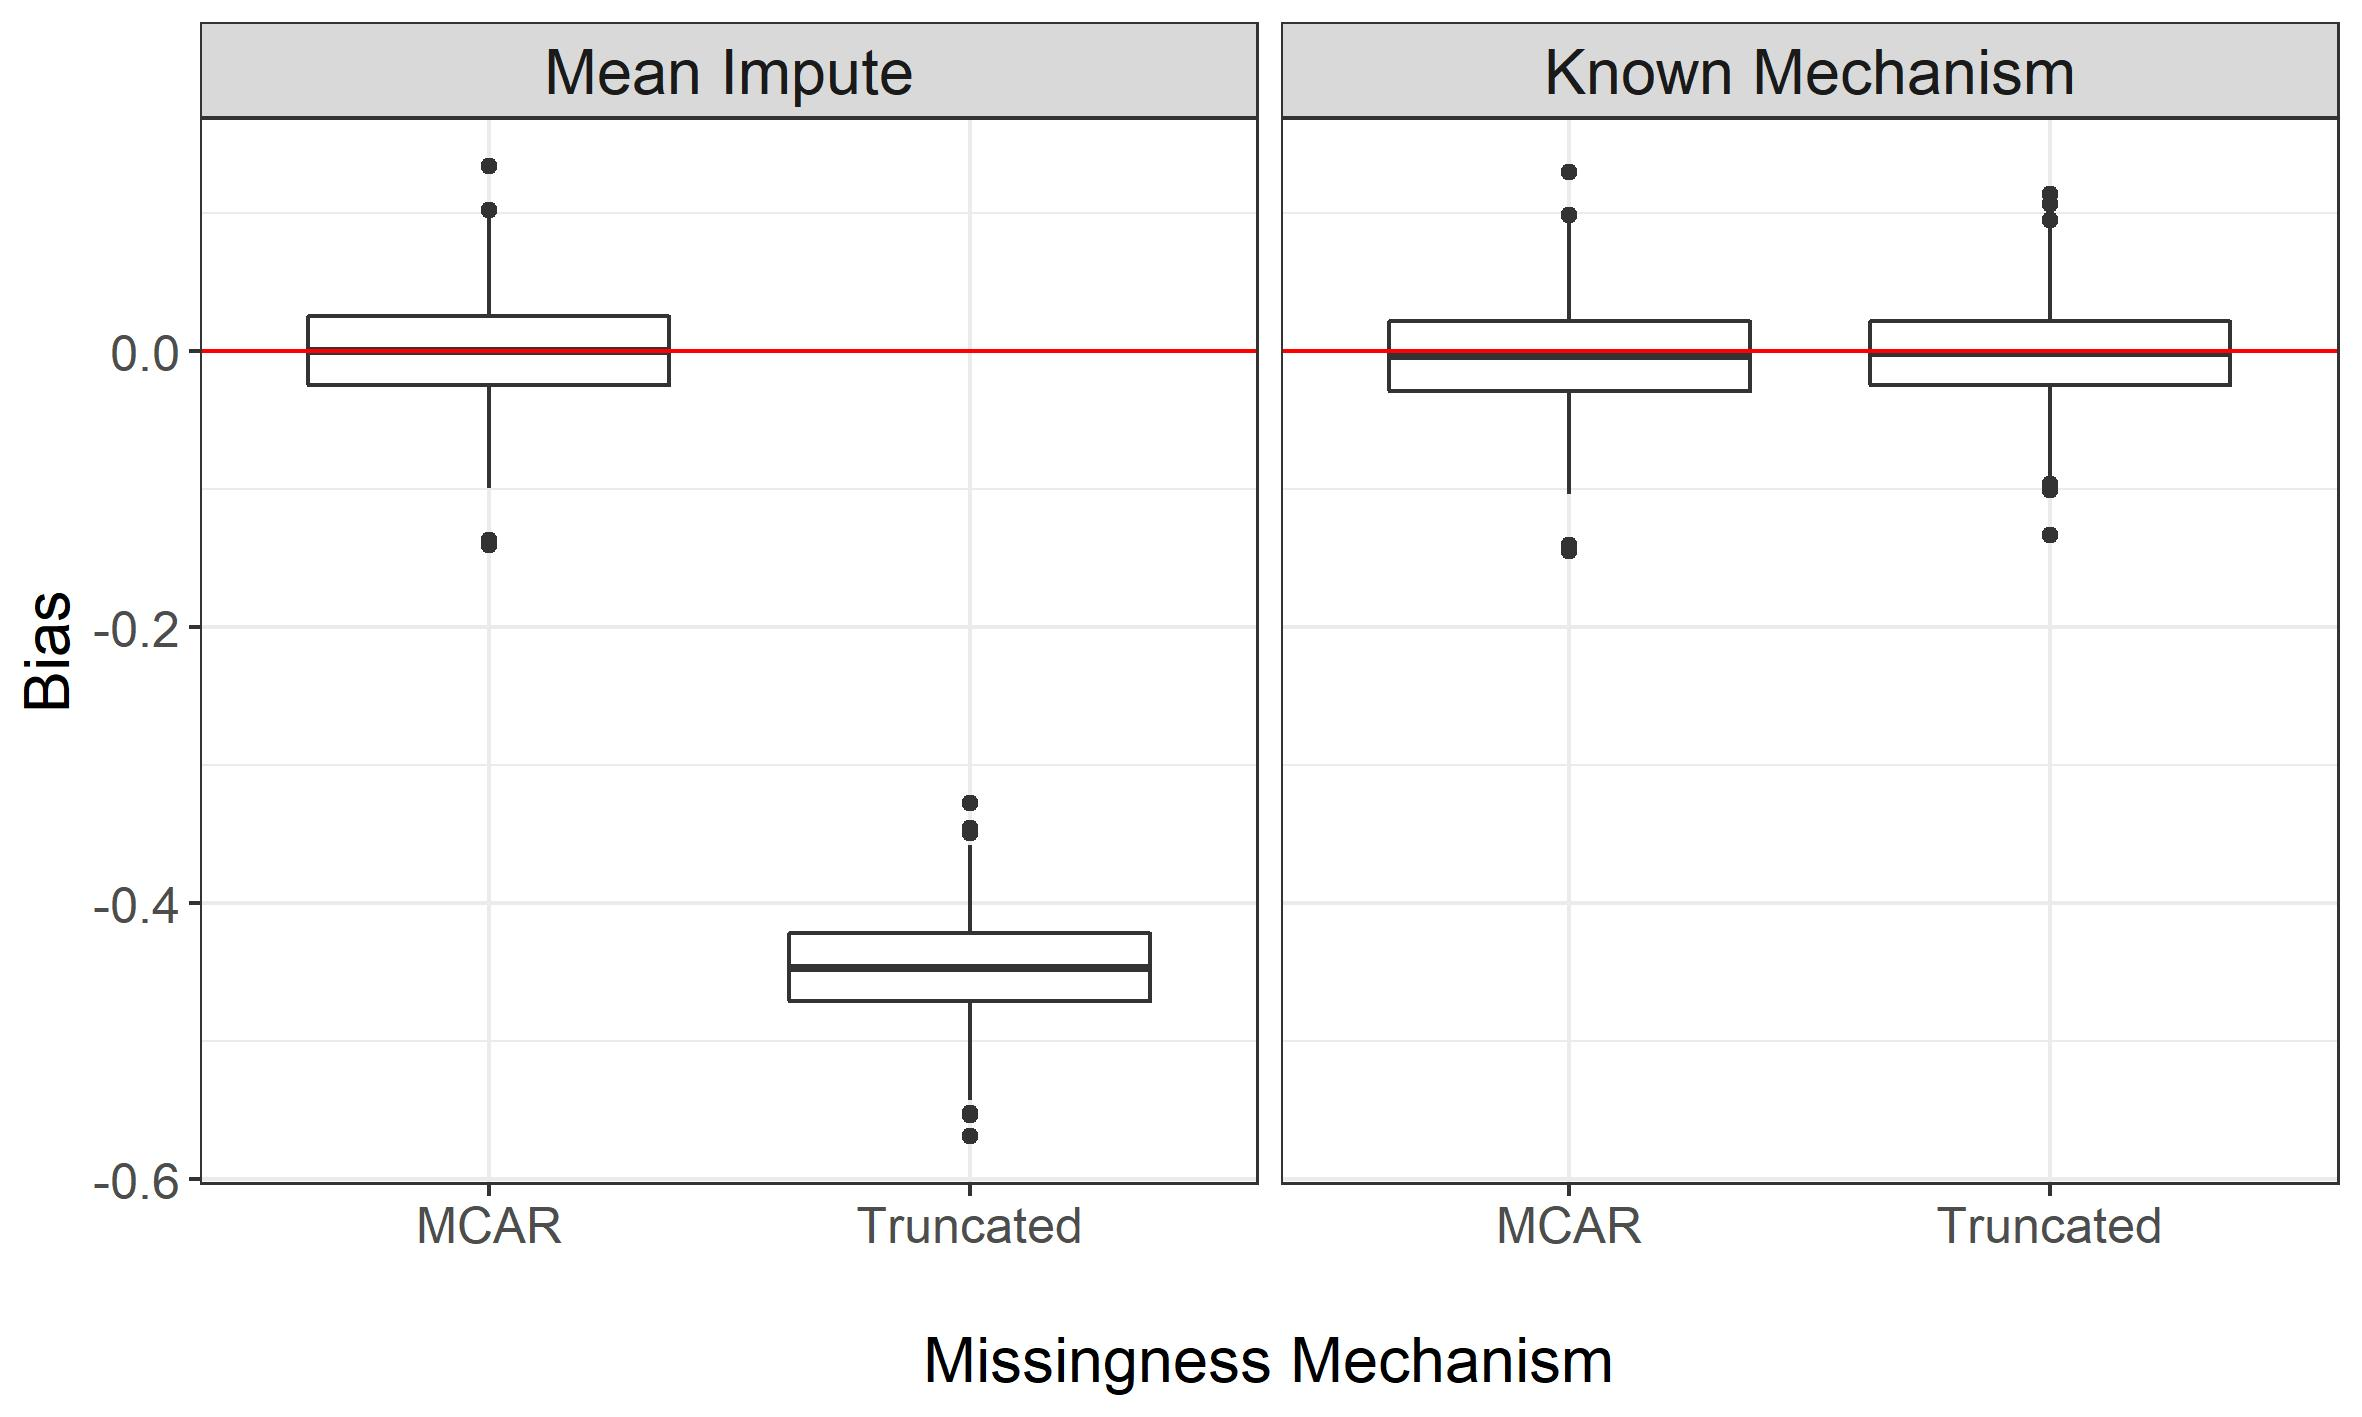
\includegraphics[width=.75\textwidth]{images/plot_bias_2.jpg}
    \end{figure}
\end{frame}

\begin{frame}{Modeling the Missingness Mechanism}
    \noindent\begin{minipage}[t]{0.48\linewidth}
    \begin{figure}
        \tikz{
        % nodes
        \node[latent] (Y) {$\underset{[p]}{\boldsymbol Y}$};%
        \node[obs, right= of Y] (M) {$\underset{[p]}{\boldsymbol M}$};%
        \node[latent,above=of Y] (Z) {$\underset{[q]}{\boldsymbol Z}$}; %
        \node[const,left = of Z] (parY) {$\boldsymbol \Lambda, \boldsymbol\mu, \boldsymbol \psi$}; %
        \node[const,right = of Z, xshift = +1.5cm] (parM) {$\widetilde{\boldsymbol \Lambda}, \widetilde{\boldsymbol\mu}$}; %
        \node[obs, below= of Y] (Yobs) {$\underset{[p]}{\boldsymbol Y^{obs}}$}; 
        % plate
        \plate [inner sep=.3cm,xshift=.02cm,yshift=.2cm] {plate1} {(Z)(Y)(M)(Yobs)} {$n$}; %
        % edges
        \edge{Z,parY}{Y};
        \edge{Z, parM}{M};
        \edge{Y, M}{Yobs};
        }
        \caption{Generative model of the data and \\missingness mechanism.}
    \end{figure}
    \end{minipage}
    \fontsize{10pt}{10}\selectfont
    \noindent\begin{minipage}[t]{0.48\linewidth}
\vspace{1cm}
\noindent \textbf{Assumptions}: for $j, j'=1, \dots, p$, 
\vspace{.5cm}
    \begin{itemize}
        \item $Y_j^{obs} \perp Y_{j'}^{obs}|\boldsymbol Z$ whenever $j\neq j'$,
        \item $Y_j^{obs}|\boldsymbol Z = \boldsymbol z \sim N(\boldsymbol z^\top \boldsymbol \Lambda_{j\cdot} + \mu_j,\, \psi_j)$,
        \vspace{.3cm}
        \item $M_{j} \perp M_{j'}|\boldsymbol Z$ whenever $j\neq j'$,
        \item $M_{j}|\boldsymbol Z = \boldsymbol z \sim \text{Bernoulli}(\text{sigmoid}(\boldsymbol z^\top \widetilde{\boldsymbol \Lambda}_{j\cdot} + \widetilde{\mu}_j))$.
    \end{itemize}   
    \begin{align*}
    \end{align*}
    \end{minipage}
\end{frame}

\begin{frame}{Bias Correction with Estimated Missingness Mechanism}
    \begin{figure}
        \centering
        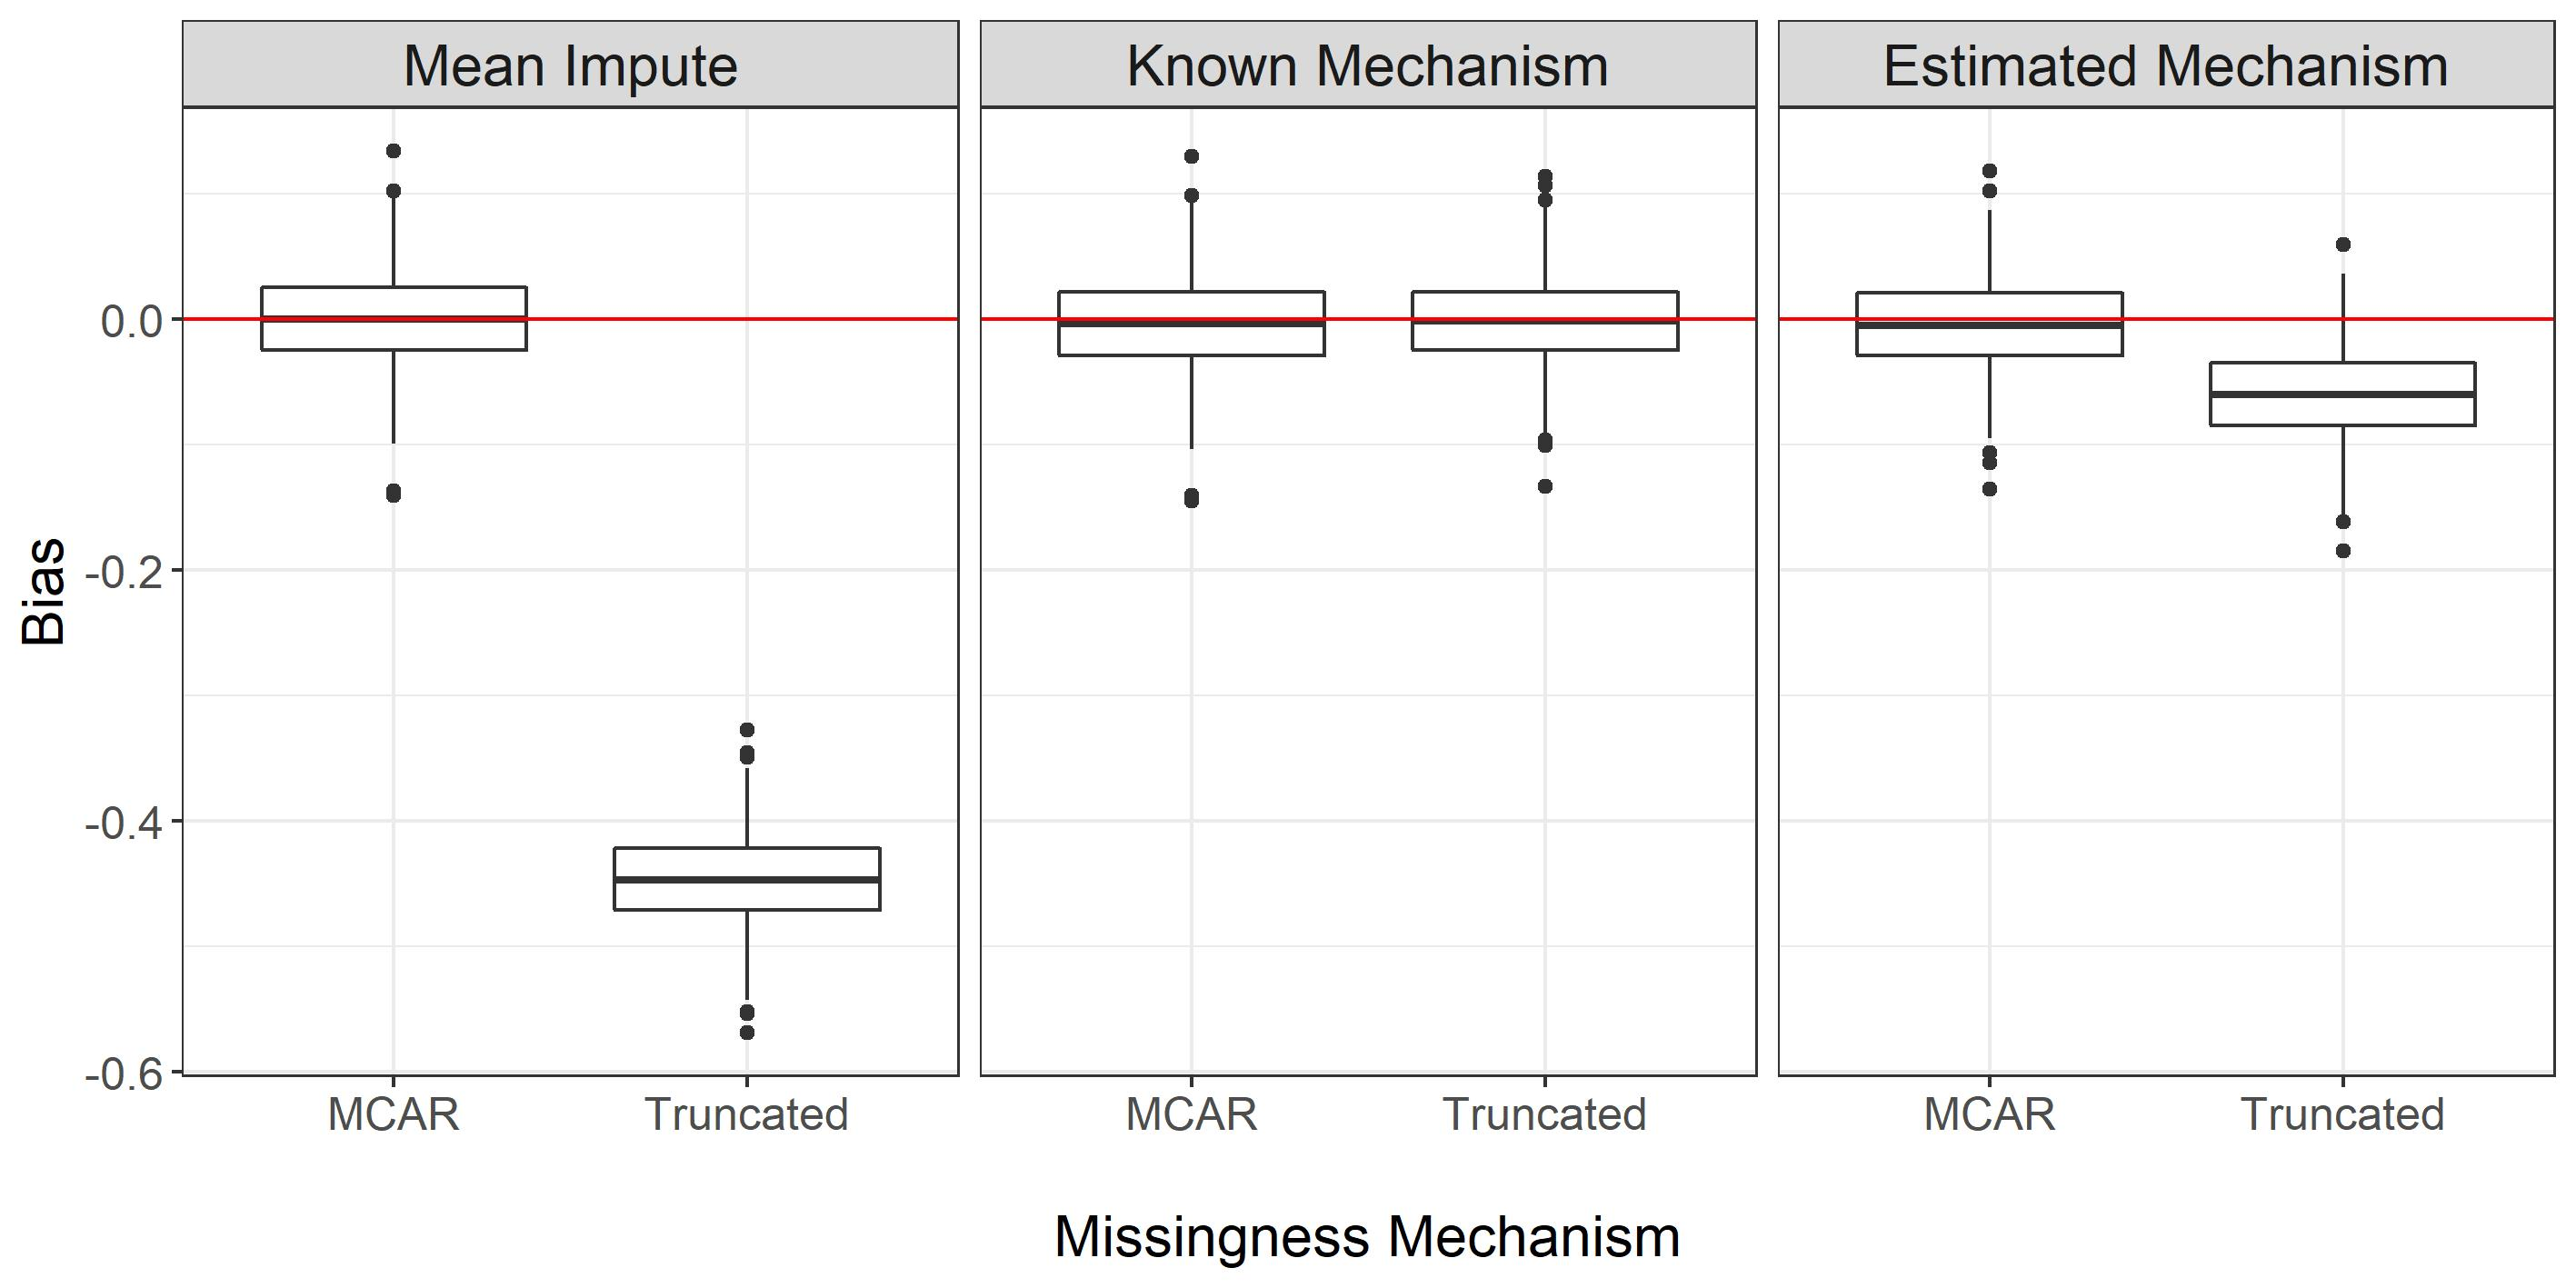
\includegraphics[width=.95\textwidth]{images/plot_bias_3.jpg}
    \end{figure}
\end{frame}
\end{document}

